\section{Übung - Analytische Funktionen}
\label{sec:uebung_07}

% ##########################################################################
% ############################### Aufgabe 01 ###############################
% ##########################################################################
\label{subsec:uebung_07.aufgabe_01}
\subsection{Aufgabe}
Zeige für jede Bestellposition die insgesamt in der Produktoberkategorie (Parentcategory) abgesetzte Menge.

\begin{figure}[H]
  \centering
  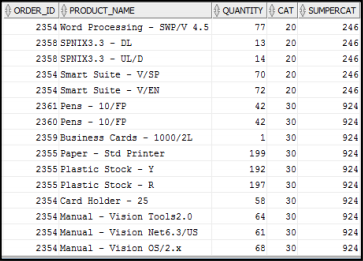
\includegraphics[width=1\textwidth]{img//uebung_07_-_aufgabe_01.png}
  \label{img:uebung_07_-_aufgabe_01}
\end{figure}

\subsubsection*{Lösung}
\label{subsubsec:uebung_07.aufgabe_01.loesung}
\inputsql{./loesungen/uebung_07/uebung_07_-_aufgabe_01.sql}


% ##########################################################################
% ############################### Aufgabe 02 ###############################
% ##########################################################################
\label{subsec:uebung_07.aufgabe_02}
\subsection{Aufgabe}
Klassifiziere die Departments nach dem durchschnittlichen Gehalt der Mitarbeiter, die in jenem Department arbeiten, in drei Klassen.

\begin{table}[H]
  \centering
  \begin{tabular}{|l|l|l|l|}
    \hline
    \textbf{DEPT\_ID} & \textbf{DEPT\_NAME}  & \textbf{AVG\_SAL} & \textbf{CLASS} \\
    \hline
    140               & Control And Credit   & 0                 & 1              \\
    260               & Recruiting           & 0                 & 1              \\
    150               & Shareholder Services & 0                 & 1              \\
    160               & Benefits             & 0                 & 1              \\
    $[$\dots$]$       &                      &                   &                \\
    20                & Marketing            & 9500              & 3              \\
    70                & Public Relations     & 10000             & 3              \\
    110               & Accounting           & 10154             & 3              \\
    90                & Executive            & 19333,33          & 3              \\
    \hline
  \end{tabular}
\end{table}

\subsubsection*{Lösung}
\label{subsubsec:uebung_07.aufgabe_02.loesung}
\inputsql{./loesungen/uebung_07/uebung_07_-_aufgabe_02.sql}


% ##########################################################################
% ############################### Aufgabe 03 ###############################
% ##########################################################################
\label{subsec:uebung_07.aufgabe_03}
\subsection{Aufgabe}
Welche sind die Top 4 Produktkategorien, gemessen am Umsatz, für alle Bestellungen aus dem Jahr 2014 die an Kunden aus Brasilien gingen?

\begin{figure}[H]
  \centering
  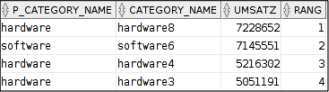
\includegraphics[width=1\textwidth]{img//uebung_07_-_aufgabe_03.png}
  \label{img:uebung_07_-_aufgabe_03}
\end{figure}

\subsubsection*{Lösung}
\label{subsubsec:uebung_07.aufgabe_03.loesung}
\inputsql{./loesungen/uebung_07/uebung_07_-_aufgabe_03.sql}


% ##########################################################################
% ############################### Aufgabe 04 ###############################
% ##########################################################################
\label{subsec:uebung_07.aufgabe_04}
\subsection{Aufgabe}
Liste die Umsätze der einzelnen Monate für 2015 auf. Dabei sollen zusätzlich die laufende Summe und der durchschnittliche Umsatz, berechnet aus dem vorherigen, aktuellen sowie nachfolgendem Monat, ausgegeben werden.

\begin{figure}[H]
  \centering
  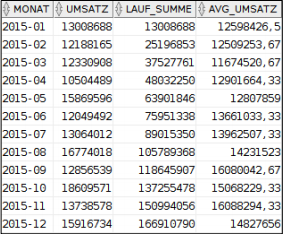
\includegraphics[width=1\textwidth]{img//uebung_07_-_aufgabe_04.png}
  \label{img:uebung_07_-_aufgabe_04}
\end{figure}

\subsubsection*{Lösung}
\label{subsubsec:uebung_07.aufgabe_04.loesung}
\inputsql{./loesungen/uebung_07/uebung_07_-_aufgabe_04.sql}


% ##########################################################################
% ############################### Aufgabe 05 ###############################
% ##########################################################################
\label{subsec:uebung_07.aufgabe_05}
\subsection{Aufgabe}
Erzeuge eine Ausgabe mit den Spalten COUNTRY\_NAME, CHANNEL\_DESC, SALES\$, RANG indem für die Vertriebskanäle alle Umsätze, die darüber gemacht wurden von März bis Juni 2008 aufgelistet und in der Spalte RANG den Rang innerhalb der Vertriebskanäle für das jeweilige Land vermerkt ist.

\begin{table}[H]
  \centering
  \begin{tabular}{|l|l|l|l|}
    \hline
    \textbf{COUNTRY} & \textbf{CHANNEL\_DESC} & \textbf{SALES\$} & \textbf{RANG}  \\
    \hline
    Argentina        & Direct Sales           & 291299           & 1              \\
    Argentina        & Partners               & 100131           & 2              \\
    Argentina        & Catalog                & 57064            & 3              \\
    Australia        & Tele Sales             & 717783           & 1              \\
    Australia        & Internet               & 508367           & 2              \\
    Australia        & Partners               & 452358           & 3              \\
    Australia        & Catalog                & 175854           & 4              \\
    Australia        & Direct Sales           & 47058            & 5              \\
    Belgium          & Partners               & 661416           & 1              \\
    Belgium          & Catalog                & 448693           & 2              \\
    Belgium          & Direct Sales           & 144147           & 3              \\
    $[$\dots$]$      &                        &                  &                \\
    \hline
  \end{tabular}
\end{table}

\subsubsection*{Lösung}
\label{subsubsec:uebung_07.aufgabe_05.loesung}
\inputsql{./loesungen/uebung_07/uebung_07_-_aufgabe_05.sql}


% ##########################################################################
% ############################### Aufgabe 06 ###############################
% ##########################################################################
\label{subsec:uebung_07.aufgabe_06}
\subsection{Aufgabe}
Welche Produkte wurden häufiger abgesetzt als der Durchschnitt der Produkte innerhalb der jeweiligen Produktoberkategorie (Hardware, Software,…)?

\subsubsection*{Lösung}
\label{subsubsec:uebung_07.aufgabe_06.loesung}
\inputsql{./loesungen/uebung_07/uebung_07_-_aufgabe_06.sql}
